% Source: Notion page “6. 大模型语义理解设计”. Generated without rewriting its content.
\chapter{大模型语义理解设计}

轻量级行为识别模型主要基于人体骨架序列进行时空图建模，通过 GCN 学习关节之间的空间关系以及动作随时间变化的动态模式。该方法能够有效提取速度、姿态变化、关节协同运动等判别性特征，对于步行、奔跑等具有明显运动模式差异的行为具有较好的识别能力。

然而，对于“玩闹追逐与冲突追逐”“玩闹推搡与冲突推搡”等细粒度行为，其底层人体运动模式具有较高相似性。此时，仅依赖 GCN 从骨架序列中学习得到的时空判别特征，可能难以充分刻画人物之间的交互性质和行为语义，从而导致类别混淆。

因此，本项目引入多模态大模型作为语义教师，语义教师采用与具体模型解耦的接口设计。系统仅要求所接入模型具备骨架时序理解、结构化文本理解、封闭类别推理以及结构化结果生成能力。当前实现采用 Qwen3-VL-8B-Instruct 作为推理后端，在保持输入输出协议不变的情况下，也可替换为其他具备相同能力的大模型。多模态大模型推理的整体流程如下。

\begin{figure}[htbp]
\centering
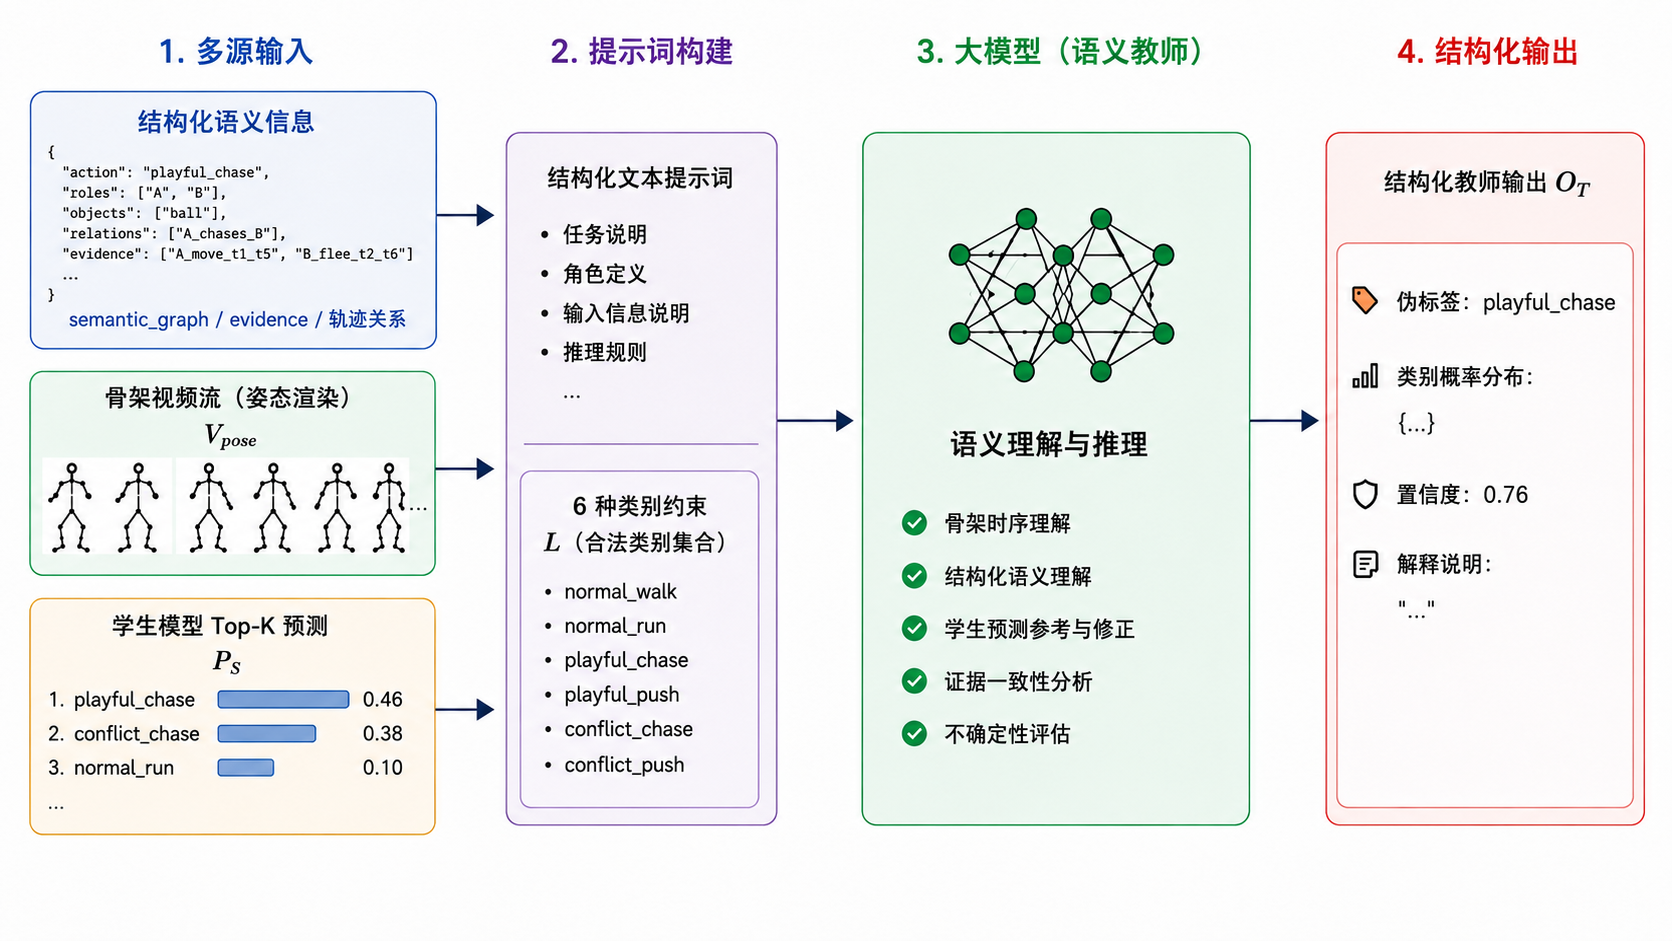
\includegraphics[width=0.96\linewidth,keepaspectratio]{figures/notion_image_03.png}
\end{figure}

注：在实际构建中，我们可能并没有三种输入数据，而我们的大模型推理模块则会采用实际可获得的数据类型进行推理。

\section{多源输入}

语义教师并非单独依据学生模型的分类结果重新判断，而是同时接收骨架视频流、结构化语义信息和学生模型预测结果，从不同信息层面对同一行为片段进行描述。

整体输入定义为：

\[
I_T=
\left\{
V_{\mathrm{pose}},
G_{\mathrm{sem}},
P_S
\right\}
\]

三类信息具有不同作用。

\subsection{结构化语义信息}

原始 RGB 视频仅在边缘端用于人体检测与姿态估计，不作为教师模型输入。系统根据骨架序列进一步构造结构化语义信息，用于描述人物运动状态和交互关系。

结构化语义信息可包括人物数量、姿态质量、运动速度、人物间距离变化、接近或远离关系、主要肢体运动以及其他由骨架序列能够可靠提取的行为特征。

这些信息以结构化字段或文本形式提供给教师模型，使大模型能够在不访问原始 RGB 视频的情况下结合骨架运动和学生模型预测进行语义判断。

\subsection{骨架视频流}

骨架视频由人体姿态估计结果渲染得到，以连续视频形式显式展示人体关键点及骨骼连接随时间的变化。

表示为：

\[
V_{\mathrm{pose}}
=
\{
S_1,S_2,\ldots,S_N
\}
\]

其中 \(S_t\) 为第 \(t\) 帧对应的骨架可视化结果。

与重新构造速度、人物距离、接近关系等人工语义规则不同，本方案直接将骨架序列渲染为视觉信息交给多模态大模型，使模型自行理解：

\begin{itemize}
\item 人体姿态变化；
\item 肢体运动幅度；
\item 人物运动方向；
\item 多人之间的位置关系；
\item 行为随时间的变化过程。
\end{itemize}

这样可以保持清晰的模块职责：

\[
\boxed{
\text{姿态模块负责提取人体骨架}
}
\]

\[
\boxed{
\text{大模型负责理解骨架运动所对应的行为语义}
}
\]

避免在大模型之前再次建立一套人工规则式行为分析模块。

当前工程的教师推理接口已经将姿态渲染视频作为 \(e_v\)ideo 传入模型，并在教师后端完成视频解码与输入构造。

教师推理阶段以骨架视频和结构化语义信息作为互补输入：骨架视频侧重人体运动结构，结构化语义信息用于补充人物交互关系、姿态质量以及运动统计等信息。

\subsection{学生模型 Top-KK 预测}

学生模型已经完成基础行为识别，因此教师模型无需忽略已有结果从零开始分类，而是将学生模型的 Top-KK 预测作为候选参考。

定义：

\[
P_S=
\{
(y_1,p_1^S),
(y_2,p_2^S),
\ldots,
(y_K,p_K^S)
\}
\]

其中：

\[
\ge p_2^S\ge\cdots\ge p_K^S
\]

例如：

\begin{NotionCode}[plain text]
playful_chase   0.46
conflict_chase  0.38
normal_run      0.10
...
\end{NotionCode}

这类结果可以直接反映学生模型当前主要在哪些类别之间产生混淆。

但学生预测只作为大模型的参考信息，不能作为确定标签。当前代码在构造教师 Prompt 时明确规定：

\begin{NotionCode}[plain text]
Student probabilities are a fallible hint and may be corrected.
\end{NotionCode}

即学生模型预测可能存在错误，教师可以根据骨架运动和结构化语义证据进行修正。

因此，多源输入的本质可以概括为：

\[
\boxed{
\text{结构化语义信息}
+
\text{骨架运动信息}
+
\text{学生候选判断}
}
\]

三者分别提供交互语义、人体运动模式以及轻量模型已有判别结果，共同组成大模型进行高层行为理解的输入基础。

\section{提示词构建}

多模态大模型本质上具有开放式视频理解和文本生成能力，而校园行为识别属于严格的封闭集合分类任务。因此，仅将视频输入模型并询问“这是什么行为”无法保证模型按照系统规定的类别和格式进行输出。

为此，本系统通过结构化 Prompt 明确规定教师模型的角色、识别任务、合法类别、学生预测使用方式、事实约束以及输出格式。

Prompt 与骨架视频、结构化语义信息共同构成教师模型完整输入：

\[
X_T=
\left[
V_{\mathrm{pose}},
G_{\mathrm{sem}},
\mathcal P
\right]
\]

其中 Prompt \(\mathcal P\) 内部进一步包含：

\[
\mathcal P=
\{
\mathcal P_{\mathrm{role}},
\mathcal P_{\mathrm{task}},
\mathcal P_{\mathrm{student}},
\mathcal P_{\mathrm{label}},
\mathcal P_{\mathrm{rule}},
\mathcal P_{\mathrm{output}}
\}
\]

\subsection{教师角色定义}

首先将模型角色限定为封闭集合视频行为分析中的弱监督教师，而不是开放式视频问答模型。

当前工程中真实使用的角色定义为：

\begin{NotionCode}[plain text]
You are a weak-supervision teacher for closed-set video behavior analysis.
\end{NotionCode}

这种角色定义明确了两个边界：

一方面，模型的任务是分类和语义判断，而不是生成任意视频描述；另一方面，教师模型的输出将作为后续协同决策和伪标签生成的信息来源，因此需要保持稳定的类别空间和输出结构。

\subsection{六分类类别约束}

对于当前 Campus6 任务，合法类别集合定义为：

\[
L=
\{
\text{normal\_walk},
\text{normal\_run},
\text{playful\_chase},
\text{playful\_push},
\text{conflict\_chase},
\text{conflict\_push}
\}
\]

Prompt 将完整标签集合直接提供给教师模型，并规定：

\begin{NotionCode}[plain text]
label must be selected from Allowed labels.
\end{NotionCode}

即：

\[
T\in L
\]

这样可以避免通用大模型输出诸如“running after someone”“fighting”“playing”等虽然自然语言上合理、但无法直接参与系统计算的开放式标签。

\subsection{学生预测使用约束}

学生 Top-KK 分布通过结构化文本输入 Prompt。

当前代码中的教师 Prompt Payload 包括：

\begin{NotionCode}[plain text]
{
  "sample_id":"...",
  "task":"...",
  "semantic_graph": {...},
  "student_distribution": {...}
}
\end{NotionCode}

其中 \(t_d\)istribution 即学生模型给出的候选类别概率。

在当前方案中，\(c_g\)raph 作为结构化语义信息的一部分继续作为核心教师输入，Prompt 同时保留样本信息、任务定义和学生预测；骨架信息通过 \(e_v\)ideo 提供给大模型。

学生预测对应的规则仍然保留：

\begin{NotionCode}[plain text]
Student probabilities are a fallible hint and may be corrected.
\end{NotionCode}

因此，大模型不会简单执行：

\[
y_T=y_S
\]

而是根据视觉信息重新判断：

\[
\left(
V_{\mathrm{rgb}},
V_{\mathrm{pose}},
P_S
\right)
\]

\subsection{事实约束与幻觉抑制}

行为识别场景中，大模型容易根据动作外观进一步推测人物意图、情绪或者未实际观察到的身体接触，从而产生超出视频证据范围的判断。

当前工程 Prompt 对这一问题进行了明确限制：

\begin{NotionCode}[plain text]
Use only facts present in INPUT.
Do not invent intent, impact force, fear, attacks,
defense, or contact.

Mark unavailable evidence as unknown.
\end{NotionCode}

即教师模型只能依据实际视觉输入和系统提供的信息作出判断，未观察到的信息必须视为未知。

这一规则对于“嬉戏—冲突”类细粒度行为尤为重要。模型不能因为运动幅度较大就自行补充“攻击意图”，也不能因为人物距离较近就自动认定存在身体接触。

\subsection{当前 Prompt 模板}

结合当前工程实现，其核心 Prompt 可以整理为：

\begin{NotionCode}[plain text]
You are a weak-supervision teacher for closed-set video behavior analysis.

Prompt version: campus6-v1.0

Task: {task}

Allowed labels:
[
  "normal_walk",
  "normal_run",
  "playful_chase",
  "playful_push",
  "conflict_chase",
  "conflict_push"
]

Rules:
- Use only facts present in INPUT.
- Do not invent intent, impact force, fear, attacks,
  defense, or contact.
- Mark unavailable evidence as unknown.
- Student probabilities are a fallible hint and may be corrected.
- Return one JSON object only, matching teacher_output.v1.
- label must be selected from Allowed labels.
- distribution probabilities must sum to 1.
- label must be the argmax of distribution.
- confidence must equal distribution[label].

INPUT:
{
  "sample_id": "{sample_id}",
  "task": "{task}",
  "student_distribution": {
      ...
  }
}

OUTPUT KEYS:
schema_version,
sample_id,
label,
distribution,
confidence,
reason
\end{NotionCode}

该模板是在当前代码 Prompt 基础上，按照骨架视频流 + 结构化语义信息方案整理后的教师输入形式。当前代码中的原始版本还包含 \(c_g\)raph、evidence、\(r_e\)vidence 和 \(s_r\)eview 等字段；按照本章新的简化设计，可将主要输出聚焦于伪标签、类别分布、置信度和解释信息。

因此，Prompt 在系统中的作用可以总结为：

\[
\boxed{
\text{开放式多模态模型}
\xrightarrow{\text{Prompt约束}}
\text{封闭集合行为语义教师}
}
\]

\section{大模型推理}

完成多源输入和 Prompt 构造后，骨架视频流、结构化语义信息和学生候选概率共同输入大模型。

语义教师的推理过程表示为：

\[
Z_T=
F_T
\left(
V_{\mathrm{pose}},
G_{\mathrm{sem}},
P_S,
\mathcal P,
L
\right)
\]

其中 \(Z_T\) 表示大模型生成的原始语义结果。

大模型主要完成三个层面的联合理解。

\subsection{结构化交互语义理解}

结构化语义信息由边缘端根据骨架序列构造，用于描述人物数量、人物间距离变化、运动方向、姿态质量以及主要肢体运动等信息。大模型结合这些结构化证据，对人物交互关系进行高层语义判断。

\subsection{骨架运动时序理解}

骨架视频去除了大量背景和外观信息，将大模型注意力集中到人体关节及其运动变化上。

因此骨架流主要提供：

\[
\text{人体姿态}
+
\text{肢体运动}
+
\text{整体位移}
+
\text{多人相对运动}
\]

等信息。

结构化语义信息与骨架视频具有互补性：前者用于表达可从骨架可靠提取的人物交互关系和运动统计，后者用于保留连续的人体姿态与运动结构。联合使用两类信息，可以降低单一信息来源对模型判断的影响。

\subsection{学生预测参考与语义修正}

学生模型输出 \(P_S\) 进一步向大模型提供候选类别范围。

例如：

\[
\text{playful\_chase})=0.46
\]

\[
\text{conflict\_chase})=0.38
\]

说明学生模型已经基本判断当前属于 chase 类行为，但无法稳定区分嬉戏追逐和冲突追逐。

此时，大模型不需要重新在完全开放的行为空间进行搜索，而可以重点判断：

\[
\text{playful\_chase}
\quad\text{vs.}\quad
\text{conflict\_chase}
\]

并根据骨架运动和结构化语义信息重新调整类别概率。

因此教师模型承担的是：

\[
\boxed{
\text{学生候选结果}
+
\text{骨架语义证据}
\rightarrow
\text{语义修正}
}
\]

而不是简单复制学生模型结果。

大模型最终形成六类行为上的教师分布：

\[
P_T=
\left[
p_1^T,
p_2^T,\ldots,p_6^T
\right]
\]

并选择：

\[
y_T=
\arg\max_{y_i\in L}p_i^T
\]

作为教师模型最终给出的伪标签。

\section{结构化输出}

大模型完成行为语义判断后，需要将结果转换为统一的结构化形式，才能进一步用于大小模型协同、伪标签数据构建以及后续知识蒸馏。

因此教师输出定义为：

\[
O_T=
\left(
y_T,
P_T,
C_T,
R_T
\right)
\]

其中：

\begin{itemize}
\item \(y_T\) 表示教师模型生成的伪标签；
\item \(P_T\) 表示六类行为上的概率分布；
\item \(C_T\) 表示教师模型对最终标签的置信度；
\item \(R_T\) 表示教师模型给出的简要语义解释。
\end{itemize}

\subsection{伪标签}

教师最终输出一个属于六类标签集合的类别：

\[
T\in L
\]

例如：

\begin{NotionCode}[plain text]
"label":"playful_chase"
\end{NotionCode}

该结果可作为后续伪标签数据构建的重要信息来源。

需要注意的是，大模型生成的标签并不意味着直接作为最终训练标签使用，其是否进入伪标签数据集以及如何与学生结果进行融合，由后续知识蒸馏和自进化流程负责。

\subsection{类别概率分布}

教师模型同时输出六分类概率分布：

\[
P_T=
\{
P_T(y_1),
P_T(y_2),
\ldots,
P_T(y_6)
\}
\]

经过归一化后满足：

\[
0\leq P_T(y_i)\leq1
\]

以及：

\[
\sum_{i=1}^{6}P_T(y_i)=1
\]

例如：

\begin{NotionCode}[plain text]
"distribution": {
  "normal_walk":0.01,
  "normal_run":0.04,
  "playful_chase":0.76,
  "playful_push":0.03,
  "conflict_chase":0.14,
  "conflict_push":0.02
}
\end{NotionCode}

与单一硬标签相比，完整概率分布保留了教师模型对其他类别的判断信息，在后续知识蒸馏中可以进一步作为软标签使用。

\subsection{置信度}

教师模型置信度定义为最终选中类别对应的概率：

\[
C_T=P_T(y_T)
\]

例如：

\begin{NotionCode}[plain text]
"confidence":0.76
\end{NotionCode}

同时要求：

\[
y_T=
\arg\max_yP_T(y)
\]

保证教师标签与概率分布保持一致。

\subsection{语义解释}

除分类结果外，教师模型还输出简要解释：

\begin{NotionCode}[plain text]
"reason":"..."
\end{NotionCode}

解释内容用于描述大模型综合骨架运动、结构化语义信息和学生候选结果之后形成当前判断的主要依据。

该字段主要服务于系统可解释性和结果展示，而不直接参与学生模型分类计算。

按照当前简化设计，教师的最终结构化输出可以表示为：

\begin{NotionCode}[plain text]
{
  "schema_version":"teacher_output.v1",
  "sample_id":"sample_001",
  "label":"playful_chase",
  "distribution": {
    "normal_walk":0.01,
    "normal_run":0.04,
    "playful_chase":0.76,
    "playful_push":0.03,
    "conflict_chase":0.14,
    "conflict_push":0.02
  },
  "confidence":0.76,
  "reason":"..."
}
\end{NotionCode}

由此，轻量模型负责高效率的基础行为判别，大模型则针对高混淆行为进一步融合结构化语义信息、骨架运动信息和学生候选结果完成语义判断，并以标准化结构输出教师伪标签及概率信息，为后续大小模型协同决策和知识蒸馏提供统一输入。

